%==============================================================================
%  ART-AI : Autonomous Red-Team AI
%  A reinforcement-learning agent for autonomous security testing against a
%  local, self-hosted vulnerable laboratory.
%
%  Compile:  pdflatex art-ai-thesis.tex   (run twice for ToC/refs)
%  Requires: tikz, pgfplots, booktabs, listings, hyperref, geometry
%==============================================================================
\documentclass[11pt,a4paper]{report}

\usepackage[utf8]{inputenc}
\usepackage[T1]{fontenc}
\usepackage{lmodern}
\usepackage[margin=1in]{geometry}
\usepackage{booktabs}
\usepackage{tabularx}
\usepackage{amsmath,amssymb}
\usepackage{graphicx}
\usepackage{xcolor}
\usepackage{listings}
\usepackage{tikz}
\usepackage{pgfplots}
\pgfplotsset{compat=1.17}
\usetikzlibrary{arrows.meta,positioning,shapes.geometric,fit,backgrounds,calc}
\usepackage[hidelinks]{hyperref}
\usepackage{caption}
\usepackage{enumitem}

%------------------------------------------------- colours & listing style
\definecolor{accent}{HTML}{B3412B}
\definecolor{ink}{HTML}{1F2933}
\definecolor{soft}{HTML}{F2F0E9}
\definecolor{good}{HTML}{2E7D54}
\definecolor{warn}{HTML}{A8601E}

\lstset{
  basicstyle=\ttfamily\footnotesize,
  backgroundcolor=\color{soft},
  frame=single, rulecolor=\color{ink!20},
  breaklines=true, captionpos=b,
  keywordstyle=\color{accent}\bfseries,
  commentstyle=\color{ink!60}\itshape,
  numbers=none, xleftmargin=4pt, framexleftmargin=4pt
}

\newcommand{\code}[1]{\texttt{\small #1}}

%==============================================================================
\begin{document}

%--------------------------------------------------------------- TITLE PAGE
\begin{titlepage}
\centering
\vspace*{1.2cm}

{\Huge\bfseries ART-AI\par}
\vspace{0.4cm}
{\LARGE Autonomous Red-Team AI\par}

\vspace{0.9cm}
\rule{\textwidth}{1.2pt}
\vspace{0.4cm}

{\Large\itshape Grounding a Reinforcement-Learning Attack Agent\\
in a Live Vulnerable Laboratory:\\
Correctness, Reproducibility, and the Sim-to-Real Gap\par}

\vspace{0.3cm}
\rule{\textwidth}{1.2pt}

\vspace{1.6cm}
{\large A Technical Thesis Report\par}
\vspace{0.4cm}
{\normalsize Submitted for academic review\par}

\vspace{2.2cm}
\begin{tabular}{rl}
\textbf{Author} & \rule{5.5cm}{0.4pt}\\[6pt]
\textbf{Supervisor} & \rule{5.5cm}{0.4pt}\\[6pt]
\textbf{Institution} & \rule{5.5cm}{0.4pt}\\[6pt]
\textbf{Date} & \today\\
\end{tabular}

\vfill

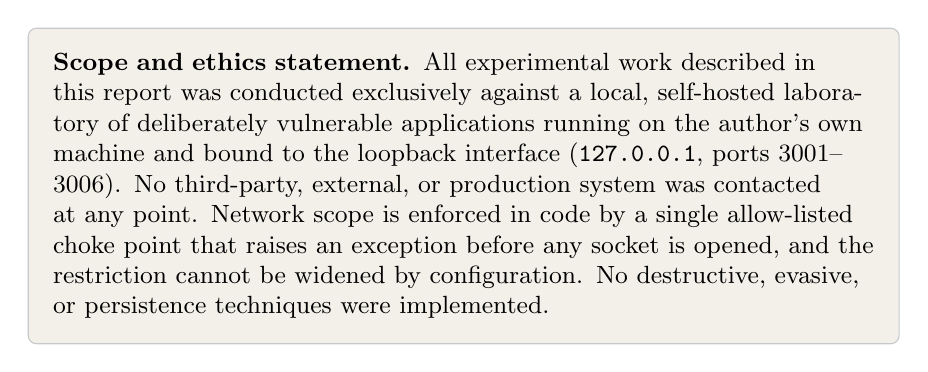
\begin{tikzpicture}
\node[draw=ink!25, fill=soft, rounded corners=3pt, inner sep=9pt,
      text width=0.86\textwidth, align=left, font=\small] {
\textbf{Scope and ethics statement.} All experimental work described in this
report was conducted exclusively against a local, self-hosted laboratory of
deliberately vulnerable applications running on the author's own machine and
bound to the loopback interface (\code{127.0.0.1}, ports 3001--3006). No
third-party, external, or production system was contacted at any point. Network
scope is enforced in code by a single allow-listed choke point that raises an
exception before any socket is opened, and the restriction cannot be widened by
configuration. No destructive, evasive, or persistence techniques were
implemented.};
\end{tikzpicture}

\vspace{0.6cm}
\end{titlepage}

%----------------------------------------------------------------- ABSTRACT
\chapter*{Abstract}
\addcontentsline{toc}{chapter}{Abstract}

Autonomous penetration-testing agents are commonly demonstrated in simulation,
where an action's outcome is resolved by sampling a hand-chosen probability.
This report documents the conversion of one such system, \textbf{ART-AI}, from a
demonstration template into a reproducible research artifact that attacks a real
laboratory, and reports the measurements that conversion made possible.

The work proceeded in three stages. \emph{First}, the reinforcement-learning
core was repaired. The original agent lost decisively to a random baseline
(2\% versus 49\% success) because its state was a single access-level string
over four values, because a non-escalating action formed a positively-rewarded
self-loop that its Q-value diverged on, and because an Exploit-DB ``hint'' bonus
of $+100$ dominated a goal reward of $+15$ to $+60$. After reformulating the
state, bounding the reward, and correcting an applicability predicate, a tabular
double-Q learner reaches a win rate of $0.960 \pm 0.035$ over 20 seeds and
attains 93\% of an exact value-iteration optimum. \emph{Second}, two components
that reported fabricated results were replaced by measurement: a port scanner
that emitted hash-derived fake ports, and a vulnerability scanner that returned
placeholder identifiers (\code{CVE-2023-XXXXX}) for every HTTP port, including
the system's own API port. \emph{Third}, a live environment was built that is
interface-compatible with the simulator but resolves every action by issuing a
real HTTP request against the laboratory and escalating only on a deterministic
oracle verdict supported by a logged response.

Two findings follow, both of which contradict the simulator's assumptions.
(i)~Every one of twelve capability probes across six services measured an
empirical success rate of $1.000$ (Wilson 95\% CI $[0.886, 1.000]$, $M=30$),
against CVSS/EPSS-derived priors ranging from $0.126$ to $0.810$ --- an error of
roughly $8\times$ in the worst case, and in the direction that mattered most,
since the prior deemed the goal-reaching action the hardest available.
(ii)~A policy trained in simulation initially failed completely on the live
laboratory (win rate $0.000$ against a random baseline's $1.000$) because the
simulator modelled a global privilege level, whereas the laboratory comprises
independent web applications between which credentials do not transfer. Once the
state abstraction was corrected, zero-shot transfer became the strongest
configuration, reaching a win rate of $1.000$ in $5.00$ steps. The principal
sim-to-real gap was therefore located in the \emph{state abstraction}, not in
the transition probabilities --- a discrepancy that only a live environment
could expose.

All reported numbers were generated by the accompanying harness; 1{,}219--2{,}126
real HTTP requests per run are recorded in an append-only evidence log that ties
each escalation to the specific request and response that justified it.

\vspace{0.4cm}
\noindent\textbf{Keywords:} reinforcement learning, autonomous security testing,
Markov decision process, sim-to-real transfer, reproducibility, vulnerability
assessment, value iteration.

%------------------------------------------------------------------- TOC
\tableofcontents
\listoffigures
\listoftables

%==============================================================================
\chapter{Introduction}

\section{Motivation}
Penetration testing is expensive, manual, and uneven in coverage. Framing it as
a sequential decision problem is attractive: an attacker in a network occupies a
state, chooses among actions with uncertain outcomes, and seeks a goal state
(administrative control) in as few steps as possible. This is precisely a Markov
decision process (MDP), and reinforcement learning (RL) is the natural tool.

The difficulty is epistemic rather than algorithmic. An RL agent trained in a
simulator learns the simulator, and a security simulator's transition
probabilities are typically invented. If those numbers are wrong, the learned
policy is confidently wrong, and nothing in the training loop can reveal it.
This report treats that gap as the central research question rather than an
implementation detail.

\section{Starting point}
ART-AI was inherited as a demonstration template: a FastAPI backend, a React
dashboard, a Docker laboratory of vulnerable applications, and a Q-learning
agent described in its own documentation as ``Optimized Q-Learning with
Experience Replay \& Double Q-Learning''. Executing the project's own
verification script produced Table~\ref{tab:before}.

\begin{table}[h]
\centering
\caption{Verified initial state, from the project's own \code{test\_rl\_learning.py}.}
\label{tab:before}
\begin{tabular}{lrr}
\toprule
\textbf{Agent} & \textbf{Win rate} & \textbf{Mean steps} \\
\midrule
Random (no learning) & 49\% & 16.7 \\
``Optimized'' Q-learning (300 training episodes) & \textcolor{accent}{\textbf{2\%}} & 22.0 \\
\midrule
Q-table size after training & \multicolumn{2}{r}{9 entries} \\
\bottomrule
\end{tabular}
\end{table}

The trained agent was an order of magnitude worse than acting at random. The
label on the method was not the problem; the environment, the state encoding,
and the reward were.

\section{Contributions}
\begin{enumerate}[leftmargin=*]
  \item \textbf{A corrected, fully-specified MDP} with a documented state
  encoding, bounded rewards, and transition probabilities derived from published
  signals rather than hand-chosen constants (Chapter~\ref{ch:method}).
  \item \textbf{An exact optimality ceiling.} Because the MDP is small and
  explicit, value iteration yields $V^\star$, so every agent is reported as a
  regret against a true optimum rather than against another heuristic.
  \item \textbf{Replacement of two fabricating components} --- a simulated port
  scanner and a template-driven vulnerability scanner --- with evidence-backed
  measurement (Chapter~\ref{ch:honesty}).
  \item \textbf{A live environment} that satisfies the simulator's interface but
  resolves actions by real HTTP requests, with a scope choke point, deterministic
  oracles, and an append-only evidence log (Chapter~\ref{ch:live}).
  \item \textbf{A quantified sim-to-real gap}, including a negative result about
  CVE-metadata-derived dynamics and the discovery that the dominant error was in
  the state abstraction (Chapter~\ref{ch:results}).
  \item \textbf{A reproducibility path}: seeded runs, logged configuration and
  git commit, pinned dependencies, and a single command that regenerates every
  number and figure.
\end{enumerate}

\section{What this work deliberately does not claim}
This is a laboratory study. The laboratory contains six deliberately vulnerable
applications on one host; it is not a network, it has no defenders beyond a
simulated intrusion-detection probability, and its vulnerabilities are static.
Several limitations are material to the conclusions and are stated in
Chapter~\ref{ch:limits} rather than omitted.

%==============================================================================
\chapter{System Architecture}

\section{Overview}
ART-AI is a four-tier system (Figure~\ref{fig:arch}). The research contribution
lives in the two rightmost tiers; the application tiers exist to make the system
usable and to expose the measurements interactively.

\begin{figure}[h]
\centering
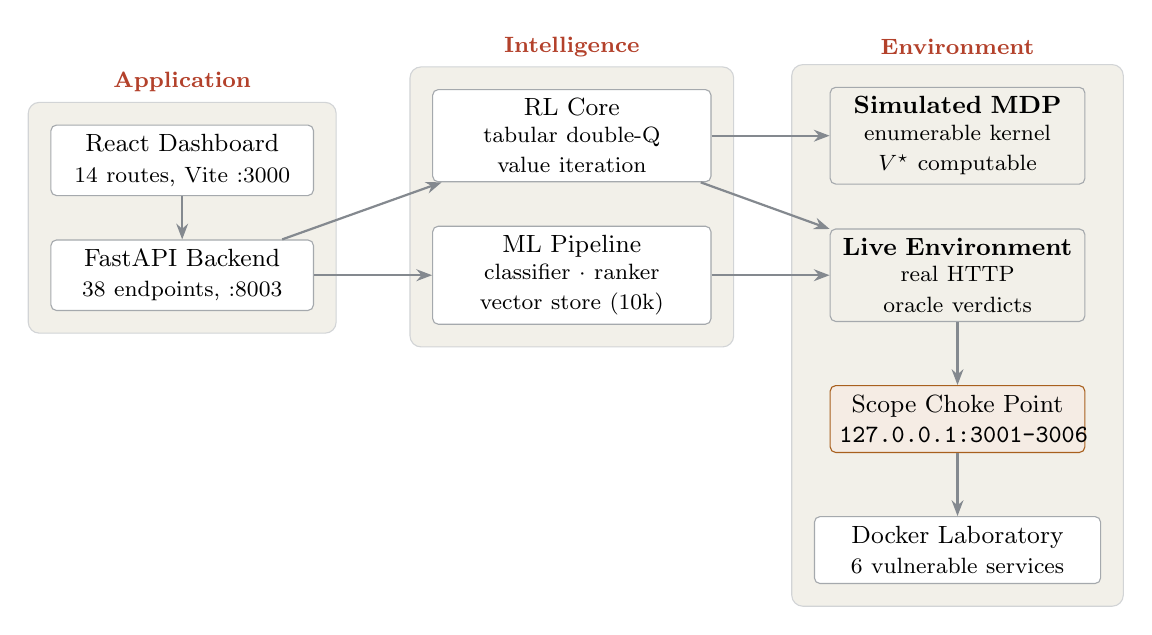
\begin{tikzpicture}[
  node distance=0.55cm,
  box/.style={draw=ink!40, fill=white, rounded corners=2pt, align=center,
              font=\small, minimum height=0.85cm, text width=3.1cm},
  tier/.style={draw=ink!20, fill=soft, rounded corners=4pt, inner sep=8pt},
  lbl/.style={font=\footnotesize\bfseries, text=accent},
  ar/.style={-{Stealth[length=2mm]}, draw=ink!55, thick}
]

% Tier 1 frontend
\node[box] (ui) {React Dashboard\\\footnotesize 14 routes, Vite :3000};
\node[box, below=of ui] (api) {FastAPI Backend\\\footnotesize 38 endpoints, :8003};

% ML
\node[box, right=1.5cm of api, text width=3.3cm] (ml)
  {ML Pipeline\\\footnotesize classifier $\cdot$ ranker\\\footnotesize vector store (10k)};

% RL
\node[box, above=of ml, text width=3.3cm] (rl)
  {RL Core\\\footnotesize tabular double-Q\\\footnotesize value iteration};

% envs
\node[box, right=1.5cm of rl, text width=3.0cm, fill=soft] (sim)
  {\textbf{Simulated MDP}\\\footnotesize enumerable kernel\\\footnotesize $V^\star$ computable};
\node[box, right=1.5cm of ml, text width=3.0cm, fill=soft] (live)
  {\textbf{Live Environment}\\\footnotesize real HTTP\\\footnotesize oracle verdicts};

% choke point
\node[box, below=0.8cm of live, text width=3.0cm, fill=warn!12, draw=warn]
  (choke) {Scope Choke Point\\\footnotesize \code{127.0.0.1:3001-3006}};

% lab
\node[box, below=0.8cm of choke, text width=3.4cm] (lab)
  {Docker Laboratory\\\footnotesize 6 vulnerable services};

\draw[ar] (ui) -- (api);
\draw[ar] (api) -- (ml);
\draw[ar] (api) -- (rl);
\draw[ar] (rl) -- (sim);
\draw[ar] (rl) -- (live);
\draw[ar] (ml) -- (live);
\draw[ar] (live) -- (choke);
\draw[ar] (choke) -- (lab);

\begin{scope}[on background layer]
\node[tier, fit=(ui)(api), label={[lbl]above:Application}] {};
\node[tier, fit=(rl)(ml), label={[lbl]above:Intelligence}] {};
\node[tier, fit=(sim)(live)(choke)(lab), label={[lbl]above:Environment}] {};
\end{scope}
\end{tikzpicture}
\caption{System architecture. The simulated and live environments expose an
identical interface, so any agent runs against either unchanged. All live
traffic passes through a single allow-listed choke point.}
\label{fig:arch}
\end{figure}

\section{What is evaluated, and what is only a demonstrator}
\label{sec:scope-of-claims}
A reviewer should not have to guess which parts of this repository carry the
results. The division is deliberate and is stated here once.

\textbf{Everything measured in this thesis is produced by \code{backend/experiments/}}
--- \code{mdp.py}, \code{grounding.py}, \code{value\_iteration.py},
\code{agents.py}, \code{live\_env.py} and the \code{run\_*.py} drivers. Those
modules compute $V^\star$, run the seeded training sweeps, drive the live lab
through the choke point, and write the result JSON and evidence logs that every
table and figure in Chapter~\ref{ch:results} is generated from. They are the
research artifact, and they are the only thing the reproduction instructions in
Appendix~\ref{app:reproduce} invoke.

\textbf{The React dashboard and the FastAPI endpoints behind it are a
demonstrator, not a contribution.} They exist to make the system legible in a
live walkthrough: to show a scan returning evidence-backed findings, or an
episode advancing step by step. They are explicitly \emph{out of scope} as an
object of evaluation, and no number in this thesis is obtained by clicking
through the UI. Two consequences follow, and are stated plainly rather than
left for a reader to discover:
\begin{itemize}
  \item The interactive attack endpoints retain the original coarse
    probability table. They were \emph{not} re-pointed at the
    CVSS/EPSS-grounded model in \code{grounding.py}, nor at the live capability
    oracles. The dashboard therefore cannot reproduce the reported results,
    and is not expected to.
  \item The LLM-backed chat endpoints are inert (no model is connected). This
    is a demonstrator gap, not a gap in the evaluation, because no result
    depends on them.
\end{itemize}
Wiring the dashboard to \code{grounding.py} and to the live oracles is a
straightforward engineering task and is listed as future work
(Section~\ref{sec:future}). It was left undone on purpose: the effort was spent
on making the measured path correct and auditable instead, and a demonstrator
that silently used different probabilities from the experiments would be a
source of confusion in exactly the place where this work is trying to be
precise.

\section{The dual-environment design}
The central architectural decision is that \code{AttackMDP} (simulated) and
\code{LiveAttackEnv} (real) implement the same contract: the same state tuple,
the same action names, the same bounded reward, and the same
\code{step(s, a, rng)} signature. Consequences:

\begin{itemize}[leftmargin=*]
  \item Every agent runs against both without modification, so sim-to-real
  transfer is measured rather than approximated.
  \item The simulator retains an enumerable transition kernel, so $V^\star$ is
  exactly computable. The live environment deliberately raises
  \code{NotImplementedError} from \code{transitions()}: a real environment has
  no enumerable kernel, which is precisely why the simulator is retained.
  \item The \code{rng} argument is accepted by the live environment for
  signature compatibility but never decides an outcome. This is asserted by a
  test: two different seeds over the same action sequence must yield identical
  oracle verdicts.
\end{itemize}

\section{Scope enforcement}
All live traffic passes through one function. It parses the URL and compares
(host, port) against a module constant before any socket is created:

\begin{lstlisting}[language=Python, caption={The scope choke point (abridged).}]
LAB_PORTS = (3001, 3002, 3003, 3004, 3005, 3006)
LAB_HOSTS = ("127.0.0.1", "localhost")
ALLOWED   = {(h, p) for h in LAB_HOSTS for p in LAB_PORTS}

def assert_in_scope(url):
    host, port = _parse(url)
    if (host, port) not in ALLOWED:
        raise ScopeViolation(f"Refusing out-of-scope target {host}:{port}")
\end{lstlisting}

No environment variable, configuration key, or command-line flag widens
\code{ALLOWED}; changing scope requires editing the constant. A test asserts
that an out-of-scope request raises \emph{before} a socket is opened, and that
the restriction is port-specific: the system's own API port 8003 is rejected.

%==============================================================================
\chapter{Datasets and Laboratory}

\section{Exploit corpus}
The ML components are trained on a processed Exploit-DB export
(Table~\ref{tab:dataset}).

\begin{table}[h]
\centering
\caption{Processed exploit corpus (\code{data\_cache/processed\_exploits.csv}).}
\label{tab:dataset}
\begin{tabular}{lr}
\toprule
\textbf{Property} & \textbf{Value}\\
\midrule
Records & 10{,}000 \\
Attributes per record & 19 \\
Exploit type: \emph{dos} / \emph{local} / \emph{remote} & 5{,}765 / 3{,}603 / 632 \\
Top platforms (windows / linux / multiple) & 5{,}401 / 1{,}782 / 1{,}107 \\
Mean CVSS score & 5.94 \\
Records flagged \emph{verified} & \textcolor{accent}{0} \\
Vector-store dimension & 5{,}000 \\
Vector-store size on disk & 382.6\,MB \\
\bottomrule
\end{tabular}
\end{table}

\paragraph{A defect worth recording.} The \emph{verified} column is zero for
every record. The grounding formula of Section~\ref{sec:grounding} assigns this
signal a weight of $0.10$; with the column uniformly zero, that term is constant
and contributes nothing but a uniform downward shift. This is a flaw in the
corpus, not in the formula, and it is reported rather than silently removed
because it bears on the negative result of Section~\ref{sec:measured}.

\section{Derived models}
Three artifacts are trained or loaded from this corpus: a gradient-boosting
exploit-type classifier (\code{exploit\_classifier.pkl}, 1.2\,MB), a
success-probability ranker (\code{exploit\_ranker.pkl}), and a graph model
(\code{model.pt}, 3.5\,MB). Semantic retrieval uses a SentenceTransformer
(\code{all-MiniLM-L6-v2}) over the 10{,}000-entry store.

\paragraph{Reproducibility note.} \code{scikit-learn} is pinned to \textbf{1.8.0}.
The shipped \code{GradientBoostingClassifier} pickle fails to load on 1.9.0 with
\code{ModuleNotFoundError: No module named '\_loss'}, an internal reorganisation
between versions. The pin is recorded in \code{requirements.txt} with this
rationale.

\section{Vulnerable laboratory}
Six deliberately vulnerable applications run as Docker containers, each bound to
the loopback interface with a health check (Table~\ref{tab:lab}).

\begin{table}[h]
\centering
\caption{Laboratory services and the capabilities confirmed against each.}
\label{tab:lab}
\small
\begin{tabularx}{\textwidth}{llXX}
\toprule
\textbf{Port} & \textbf{Service} & \textbf{Foothold oracle} & \textbf{Privilege-escalation oracle}\\
\midrule
3001 & OWASP Juice Shop & SQLi authentication bypass yielding a decodable JWT & \code{/api/Users} returns 401 anonymously, 200 with token \\
3002 & DVWA & authenticated session; \code{/index.php} returns 200 & SQLi differential, $1 \rightarrow 5$ rows \\
3003 & Flask API (in-repo) & SQLi differential, $1 \rightarrow 4$ rows & login returns \code{role="admin"}; wrong password 401 \\
3004 & OWASP WebGoat & registration + login; own username on an authenticated page & lesson-8 SQLi, $2 \rightarrow 6$ rows \\
3005 & VAmPI & \code{/users/v1/\_debug} exposes plaintext passwords & mass assignment sets \code{admin:true} \\
3006 & bWAPP & \code{bee}/\code{bug} session reaching the portal & SQLi differential, $2 \rightarrow 17$ cells \\
\bottomrule
\end{tabularx}
\end{table}

Every oracle is a deterministic predicate on a real response, and each is paired
with a benign baseline so that success is a measured \emph{difference} rather
than an absolute judgement. Two pre-test assumptions were falsified by contact
with the running services and are recorded in Section~\ref{sec:corrections}.

%==============================================================================
\chapter{Methodology}
\label{ch:method}

\section{MDP formulation}
A state is the tuple $s = (\textit{access}, \textit{position}, \textit{discovered})$:

\begin{itemize}[leftmargin=*]
  \item $\textit{access} \in \{\textsc{none}, \textsc{user}, \textsc{admin}\}$,
  the privilege obtained. \textsc{admin} is the goal and is absorbing.
  \item $\textit{position} \in \{0,\dots,N-1\}$, the host the attacker operates
  from. \code{exploit} always acts on this host.
  \item $\textit{discovered} \subseteq \{0,\dots,N-1\}$, hosts revealed by
  reconnaissance. A host may be moved to or exploited only once discovered.
\end{itemize}

The canonical key is \code{a\{access\}|p\{position\}|d\{sorted discovered\}}, for
example \code{a1|p0|d0,1}. With $N=3$ this yields $3 \times 3 \times 2^3 = 72$
states --- small enough to enumerate, large enough to require a policy.

\paragraph{Why the original formulation failed.} The inherited code used the
access level alone as the state: four values, of which one is terminal, leaving
three. Worse, a successful \code{lateral\_movement} at the \textsc{internal}
level escalated to \textsc{internal} --- a no-op that nevertheless returned
success and collected reward. Because the state did not change, the update
bootstrapped on $\max_a Q(s,a)$ including the action being updated, producing a
positively-reinforced self-loop. The observed $Q$ value diverged to $90.89$ and
the greedy policy never attempted the only action reaching \textsc{admin}.

\begin{figure}[h]
\centering
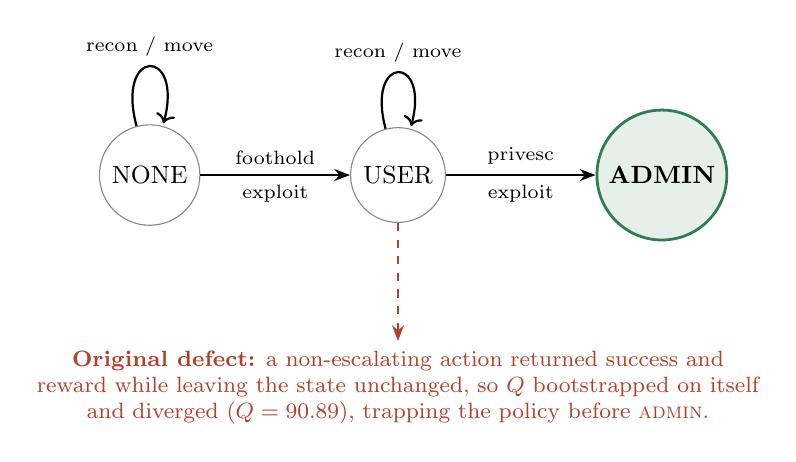
\begin{tikzpicture}[
  node distance=1.9cm,
  st/.style={circle, draw=ink!55, fill=white, minimum size=1.05cm, font=\small},
  goal/.style={circle, draw=good, fill=good!12, line width=1pt, minimum size=1.05cm, font=\small\bfseries},
  ar/.style={-{Stealth[length=2mm]}, thick},
  lp/.style={-{Stealth[length=2mm]}, thick, draw=accent}
]
\node[st] (n) {NONE};
\node[st, right=of n] (u) {USER};
\node[goal, right=of u] (a) {ADMIN};

\draw[ar] (n) -- node[above,font=\scriptsize]{foothold} node[below,font=\scriptsize]{exploit} (u);
\draw[ar] (u) -- node[above,font=\scriptsize]{privesc} node[below,font=\scriptsize]{exploit} (a);
\draw[ar] (n) edge[loop above] node[font=\scriptsize]{recon / move} (n);
\draw[ar] (u) edge[loop above] node[font=\scriptsize]{recon / move} (u);

\node[below=1.5cm of u, align=center, font=\footnotesize, text=accent]
 (bad) {\textbf{Original defect:} a non-escalating action returned success and\\
 reward while leaving the state unchanged, so $Q$ bootstrapped on itself\\
 and diverged ($Q = 90.89$), trapping the policy before \textsc{admin}.};
\draw[lp, dashed] (u) -- (bad);
\end{tikzpicture}
\caption{Privilege-escalation chain and the self-loop that defeated the original
agent.}
\label{fig:mdp}
\end{figure}

\section{Reward}
The reward is deliberately minimal and bounded:
\[
r(s,a,s') = -c_{\text{step}} + R_{\text{goal}} \cdot \mathbb{1}[s' \text{ is } \textsc{admin}],
\qquad c_{\text{step}} = 0.01,\; R_{\text{goal}} = 1.0 .
\]
With discount $\gamma = 0.95$, the discounted return rewards reaching the goal
quickly without further shaping.

\paragraph{Removal of reward hacking.} The inherited reward granted $+96$ to
$+120$ when the chosen action matched an Exploit-DB ``hint'', while reaching
\textsc{admin} --- the actual objective --- was worth $15 \cdot 2^{\Delta}$,
i.e.\ $15$ to $60$. Matching a string was therefore worth between two and eight
times more than winning the episode. The hint was removed from the reward
entirely and re-introduced only as an \emph{exploration prior}, whose value is
measured by ablation. Because it biases exploration and never the reward or the
target, it can change sample efficiency but provably cannot change the fixed
point.

\section{Data-grounded transition probabilities}
\label{sec:grounding}
The inherited \code{SUCCESS\_PROBABILITIES} were hand-chosen literals. They were
replaced by a single documented function of published signals. The CVSS v3.1
exploitability sub-score uses the official metric weights:
\[
E = 8.22 \cdot \mathrm{AV} \cdot \mathrm{AC} \cdot \mathrm{PR} \cdot \mathrm{UI},
\qquad
\hat{E} = E / E_{\max},\quad E_{\max} = 3.887 .
\]
These are combined with EPSS, an Exploit-DB verified flag, and patch age:
\[
p = \big(w_{c}\hat{E} + w_{e}\,\mathrm{EPSS} + w_{v}\,\mathrm{verified}\big)
    \cdot \underbrace{\Big(1 - 0.3 \cdot 2^{-\,\text{age}/365}\Big)}_{\text{recency}},
\qquad p \in [0.05,\, 0.95],
\]
with $w_c = 0.55$, $w_e = 0.35$, $w_v = 0.10$. The weights are stated in source
rather than hidden in a per-action table. The resulting priors appear in
Table~\ref{tab:priors}.

\begin{table}[h]
\centering
\caption{Derived priors. The asymmetry is deliberate: the cheapest foothold host
is the weakest escalation host, so an optimal policy must reposition.}
\label{tab:priors}
\begin{tabular}{lrr}
\toprule
\textbf{Host} & \textbf{Foothold $p$} & \textbf{Privesc $p$}\\
\midrule
juice-shop & 0.810 & 0.126\\
dvwa       & 0.536 & 0.384\\
flask-api  & 0.216 & 0.508\\
\bottomrule
\end{tabular}
\end{table}

\section{Agents and baselines}
\begin{itemize}[leftmargin=*]
  \item \textbf{Random} --- uniform over the action set.
  \item \textbf{Greedy-by-signal} --- a non-learning heuristic following the
  grounded signal; the ``greedy-by-CVSS'' baseline.
  \item \textbf{Tabular Q-learning} --- with independently switchable double-Q,
  experience replay, Boltzmann versus $\varepsilon$-greedy exploration, and the
  hint prior, so each is ablatable.
  \item \textbf{Value iteration} --- the exact optimum $V^\star$, computed from
  the explicit kernel. This is the ceiling, and regret is measured against it.
\end{itemize}

\section{Experimental protocol}
Twenty independent seeds derived deterministically from a master seed; 800
training episodes per run; a 15-step episode cap chosen so that win rate is
discriminating (random $\approx 0.17$, optimal $\approx 1.0$); 200 evaluation
episodes per run. Confidence intervals are $t$-based for the simulation and
Wilson for live win rates, where $N$ is small. Seed, git commit, configuration,
and library versions are written alongside every result.

%==============================================================================
\chapter{From Fabrication to Measurement}
\label{ch:honesty}

Two components reported results they had not obtained. Both were replaced. They
are documented because the failure mode --- plausible output that was never
measured --- is the central hazard in autonomous security tooling.

\section{The port scanner}
\code{recon.py} contained \code{\_simulate\_port\_scan}, which decided whether a
port was open from \code{hash(f"\{target\}:\{port\}") \% 100} and attached a
banner from a hard-coded table. Neither \code{recon.py} nor
\code{vulnerability\_scanner.py} contained a single socket call. Scanning
\code{127.0.0.1} reported ports 25 (Postfix) and 9200 (Elasticsearch), neither
of which was listening, while missing every port that was.

It was rewritten as a concurrent TCP connect scanner with real banner
acquisition. Its output now matches \code{netstat} exactly
(Table~\ref{tab:scan}), and out-of-scope targets are refused with HTTP 400.

\begin{table}[h]
\centering
\caption{Scanner output before and after, against the same host.}
\label{tab:scan}
\small
\begin{tabular}{ll}
\toprule
\textbf{Before (fabricated)} & \textbf{After (measured)}\\
\midrule
25/tcp ``Postfix smtpd'' --- \emph{not listening} & 3002 \code{Apache/2.4.25 (Debian)}\\
9200/tcp ``Elasticsearch'' --- \emph{not listening} & 3003 \code{Werkzeug/3.0.1 Python/3.11.16}\\
ports 3001--3006, 8003 --- \emph{missed} & 3005 \code{Werkzeug/2.2.3 Python/3.11.15}\\
 & 3006 \code{Apache/2.4.7 (Ubuntu)}\\
\bottomrule
\end{tabular}
\end{table}

\section{The vulnerability scanner}
\code{vulnerability\_scanner.py} mapped a service \emph{name} to a fixed list of
three findings carrying placeholder identifiers \code{CVE-2023-XXXXX},
\code{CVE-2023-YYYYY} and \code{CVE-2023-ZZZZZ}, then decided whether each was
``found'' using
\code{hash(f"\{target\}:\{service\}:\{name\}") \% 100 < probability*100}.
Consequently every HTTP port received identical findings --- including port
8003, the system's own API, which has none of them.

It was replaced by six detectors that issue real requests and report a finding
only when evidence confirms it (Table~\ref{tab:vulns}). Crucially, \textbf{no
CVE identifier is fabricated}: the \code{cve} field remains null unless a
specific CVE is genuinely known, and findings instead carry a CWE class, which
accurately describes what was observed. The reported count fell from 21
fabricated findings to 7 confirmed ones, and port 8003 is no longer flagged.

\begin{table}[h]
\centering
\caption{Confirmed findings, each with the evidence that established it.}
\label{tab:vulns}
\small
\begin{tabularx}{\textwidth}{llX}
\toprule
\textbf{Port} & \textbf{Finding (CWE)} & \textbf{Evidence}\\
\midrule
3001 & SQL Injection (CWE-89) & injected request surfaced \code{SQLITE\_ERROR}; benign did not\\
3001 & Auth Bypass (CWE-89) & token issued for \code{' OR 1=1--} with no valid password\\
3003 & SQL Injection (CWE-89) & benign query returned 2 records; injected returned 8\\
3003 & Path Traversal (CWE-22) & response contained \code{root:x:0:0:}\\
3003 & Reflected XSS (CWE-79) & marker reflected with tags unencoded\\
3003 & Default Credentials (CWE-1392) & \code{admin/admin123} authenticated as \code{role=admin}\\
3005 & Sensitive Data Exposure (CWE-200) & \code{/users/v1/\_debug} returned 83 plaintext passwords\\
\bottomrule
\end{tabularx}
\end{table}

Ports 3002, 3004 and 3006 now report \emph{zero} unauthenticated findings. This
is the correct result --- their injection points require an authenticated
session --- and is preferred to the three fabricated findings each previously
received.

%==============================================================================
\chapter{The Live Environment}
\label{ch:live}

\section{Design}
\code{LiveAttackEnv} implements the simulator's interface, but \code{exploit}
invokes a capability probe that issues real requests and escalates only on a
\code{True} oracle verdict; \code{recon} performs a real port scan, so discovery
is an observation rather than a $0.90$ constant; and a failed request is
recorded as a failed action or an episode error, never resolved by a
probability.

\begin{figure}[h]
\centering
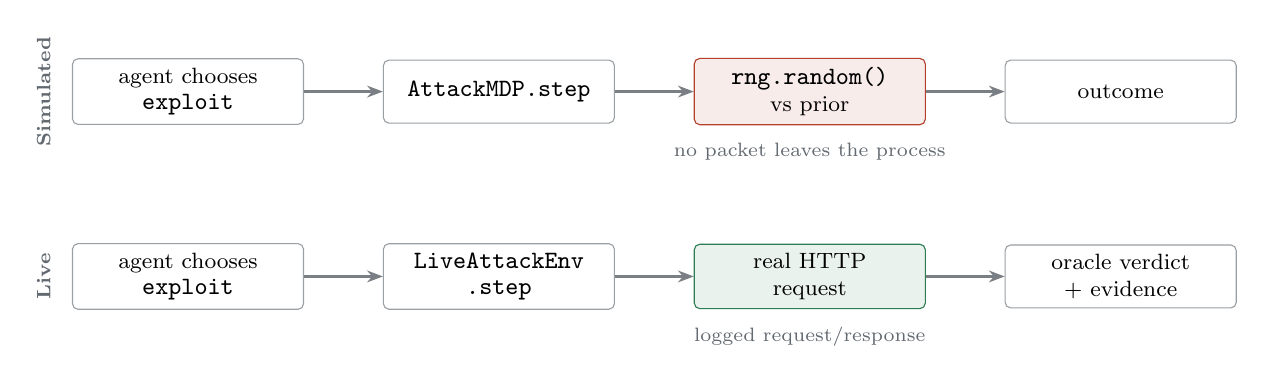
\begin{tikzpicture}[
  box/.style={draw=ink!45, fill=white, rounded corners=2pt, align=center,
              font=\footnotesize, minimum height=0.8cm, text width=2.7cm},
  ar/.style={-{Stealth[length=2mm]}, thick, draw=ink!60},
  note/.style={font=\scriptsize, text=ink!70}
]
% simulated row
\node[box] (a1) {agent chooses\\\code{exploit}};
\node[box, right=1.0cm of a1] (s1) {\code{AttackMDP.step}};
\node[box, right=1.0cm of s1, fill=accent!10, draw=accent] (r1) {\code{rng.random()}\\vs prior};
\node[box, right=1.0cm of r1] (o1) {outcome};
\draw[ar] (a1)--(s1); \draw[ar] (s1)--(r1); \draw[ar] (r1)--(o1);
\node[note, left=0.15cm of a1, rotate=90, anchor=south] {\textbf{Simulated}};

% live row
\node[box, below=1.5cm of a1] (a2) {agent chooses\\\code{exploit}};
\node[box, right=1.0cm of a2] (s2) {\code{LiveAttackEnv}\\\code{.step}};
\node[box, right=1.0cm of s2, fill=good!10, draw=good] (r2) {real HTTP\\request};
\node[box, right=1.0cm of r2] (o2) {oracle verdict\\+ evidence};
\draw[ar] (a2)--(s2); \draw[ar] (s2)--(r2); \draw[ar] (r2)--(o2);
\node[note, left=0.15cm of a2, rotate=90, anchor=south] {\textbf{Live}};

\node[note, below=0.1cm of r1] {no packet leaves the process};
\node[note, below=0.1cm of r2] {logged request/response};
\end{tikzpicture}
\caption{How an \code{exploit} action resolves in each environment. The
simulated path never contacts the network; the live path escalates only on
evidence.}
\label{fig:simlive}
\end{figure}

\section{Episode reset on stateful targets}
Reset follows a preference order. Ten of twelve capabilities use
\emph{idempotent probes} (differentials and reads repeat cleanly, requiring no
reset). The two mutating probes --- VAmPI and WebGoat registration --- use
\emph{per-episode unique identifiers}, so episodes cannot collide. No container
restart proved necessary, giving a per-episode reset cost of approximately
$0$\,s. The residual cost is accumulation: each run adds one account per
registration probe, which is harmless but should be cleared periodically.

\section{Evidence log}
Every step appends a record containing the timestamp, episode, step index, state
key, action, host, every request issued (method, URL, status, latency, length),
the oracle verdict, and the evidence string. This is what makes ``the agent
attacked the laboratory'' auditable rather than asserted:

\begin{lstlisting}[caption={An evidence record (abridged).}]
ep1 step5  a0|p0|d0 --exploit--> a1|p0|d0   host=juice-shop  verdict=True
  evidence: status=200 jwt_identity=admin@juice-sh.op|role=admin
  POST http://127.0.0.1:3001/rest/user/login -> HTTP 200  19.4ms  784B
\end{lstlisting}

%==============================================================================
\chapter{Results}
\label{ch:results}

\section{Simulation}
Table~\ref{tab:sim} reports 20 seeds $\times$ 800 episodes. The repaired agent
attains $0.960 \pm 0.035$ against a random baseline of $0.171 \pm 0.012$, and
reaches 93\% of the exact optimum.

\begin{table}[h]
\centering
\caption{Simulated results. $N=20$ seeds, mean $\pm$ 95\% CI. Regret is measured
against the exact value-iteration optimum $V^\star = 0.6772$.}
\label{tab:sim}
\begin{tabular}{lrrrr}
\toprule
\textbf{Configuration} & \textbf{Win rate} & \textbf{Steps} & \textbf{Return} & \textbf{Regret}\\
\midrule
Random                      & $0.171 \pm 0.012$ & 11.50 & $-0.003$ & 0.680\\
Greedy-by-signal            & $0.999 \pm 0.001$ & 7.49  & 0.655 & 0.022\\
\textbf{Q-learning (repaired)} & $\mathbf{0.960 \pm 0.035}$ & 7.43 & 0.631 & 0.047\\
\midrule
\multicolumn{5}{l}{\emph{Ablations}}\\
double-Q off                & $0.976 \pm 0.029$ & 7.33 & 0.647 & 0.031\\
replay off                  & $0.973 \pm 0.033$ & 7.41 & 0.641 & 0.036\\
Boltzmann (vs $\varepsilon$-greedy) & $0.973 \pm 0.027$ & 7.21 & 0.649 & 0.028\\
hint on                     & $0.978 \pm 0.027$ & 7.42 & 0.643 & 0.034\\
\midrule
Value-iteration optimum     & --- & --- & \textbf{0.677} & 0.000\\
\bottomrule
\end{tabular}
\end{table}

\paragraph{Ablations, reported honestly.} Only one technique shows a
statistically defensible benefit. Disabling experience replay raises
episodes-to-competence from $36.3 \pm 8.0$ to $73.8 \pm 22.9$; the intervals do
not overlap, so replay approximately halves the episodes required. Its effect on
final policy quality is not significant. Double-Q, Boltzmann exploration and the
hint prior all have final-regret and sample-efficiency differences whose
confidence intervals overlap the baseline: on an MDP of this size none is
justified by a measured improvement, and this is stated rather than asserted
away. The Q-table grew from 9 entries to $59.95 \pm 1.77$.

\begin{figure}[h]
\centering
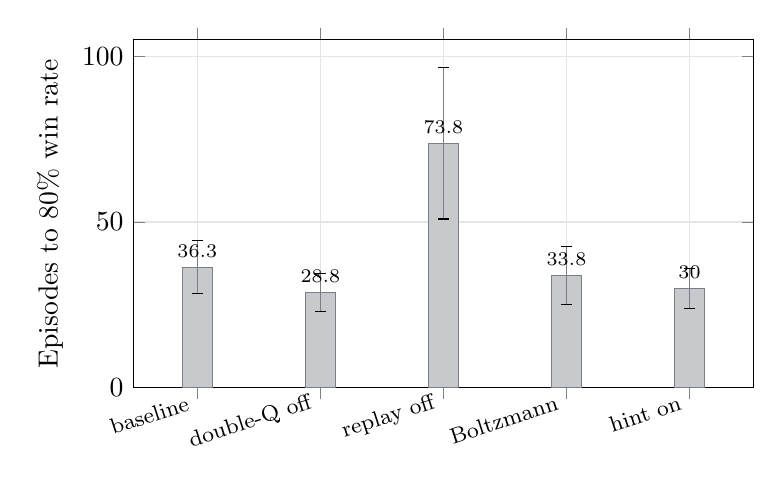
\begin{tikzpicture}
\begin{axis}[
  width=0.78\textwidth, height=6cm,
  ybar, bar width=11pt,
  ylabel={Episodes to 80\% win rate},
  symbolic x coords={baseline, double-Q off, replay off, Boltzmann, hint on},
  xtick=data, x tick label style={rotate=18, anchor=east, font=\footnotesize},
  ymin=0, ymax=105,
  error bars/y dir=both, error bars/y explicit,
  enlarge x limits=0.13,
  nodes near coords, nodes near coords style={font=\scriptsize},
  grid=major, grid style={ink!12}
]
\addplot[fill=ink!25, draw=ink!60] coordinates {
  (baseline,36.3) +- (0,8.0)
  (double-Q off,28.8) +- (0,5.7)
  (replay off,73.8) +- (0,22.9)
  (Boltzmann,33.8) +- (0,8.7)
  (hint on,30.0) +- (0,6.1)
};
\end{axis}
\end{tikzpicture}
\caption{Sample efficiency by ablation. Only removing experience replay produces
a non-overlapping interval, and it makes learning markedly slower; the remaining
techniques are statistically indistinguishable from the baseline.}
\label{fig:ablation}
\end{figure}

\section{Measured versus derived probabilities}
\label{sec:measured}
Each capability probe was executed $M=30$ times independently. Every one of the
twelve probes measured an empirical success rate of $1.000$ with Wilson 95\%
interval $[0.886, 1.000]$ (Table~\ref{tab:gap}). A later confirmation run at
$M=15$ reproduced the same rates.

\begin{table}[h]
\centering
\caption{Derived prior versus measured rate. $M=30$, Wilson 95\% CI
$[0.886, 1.000]$ throughout.}
\label{tab:gap}
\begin{tabular}{llrrr}
\toprule
\textbf{Host} & \textbf{Capability} & \textbf{Derived} & \textbf{Measured} & \textbf{Ratio}\\
\midrule
juice-shop & foothold & 0.810 & 1.000 & $1.2\times$\\
juice-shop & privesc  & \textcolor{accent}{0.126} & 1.000 & \textcolor{accent}{$7.9\times$}\\
dvwa       & foothold & 0.536 & 1.000 & $1.9\times$\\
dvwa       & privesc  & 0.384 & 1.000 & $2.6\times$\\
flask-api  & foothold & 0.216 & 1.000 & $4.6\times$\\
flask-api  & privesc  & 0.508 & 1.000 & $2.0\times$\\
\midrule
vampi, bwapp, webgoat & both & --- & 1.000 & ---\\
\bottomrule
\end{tabular}
\end{table}

\begin{figure}[h]
\centering
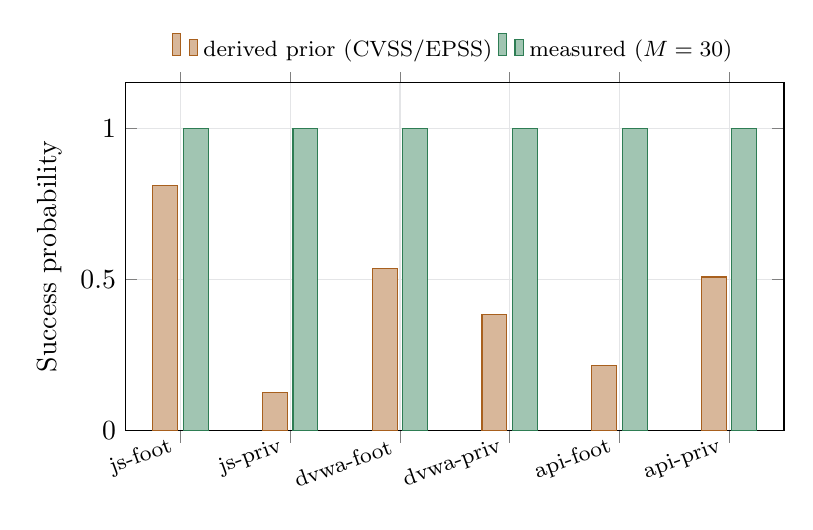
\begin{tikzpicture}
\begin{axis}[
  width=0.82\textwidth, height=6cm,
  ybar, bar width=9pt,
  ylabel={Success probability},
  symbolic x coords={js-foot, js-priv, dvwa-foot, dvwa-priv, api-foot, api-priv},
  xtick=data, x tick label style={rotate=20, anchor=east, font=\footnotesize},
  ymin=0, ymax=1.15,
  legend style={at={(0.5,1.03)}, anchor=south, legend columns=2, font=\footnotesize, draw=none},
  grid=major, grid style={ink!12}
]
\addplot[fill=warn!45, draw=warn] coordinates {
  (js-foot,0.810) (js-priv,0.126) (dvwa-foot,0.536)
  (dvwa-priv,0.384) (api-foot,0.216) (api-priv,0.508)};
\addlegendentry{derived prior (CVSS/EPSS)}
\addplot[fill=good!45, draw=good] coordinates {
  (js-foot,1.0) (js-priv,1.0) (dvwa-foot,1.0)
  (dvwa-priv,1.0) (api-foot,1.0) (api-priv,1.0)};
\addlegendentry{measured ($M=30$)}
\end{axis}
\end{tikzpicture}
\caption{Every capability is deterministic in practice, while the
CVE-metadata-derived priors span $0.126$ to $0.810$. The largest error is
juice-shop privilege escalation, under-estimated by a factor of about eight.}
\label{fig:gap}
\end{figure}

\paragraph{Interpretation (a negative result).} CVSS exploitability, EPSS and
patch age describe a \emph{population}, not an \emph{instance}. EPSS in
particular estimates the probability that a vulnerability is exploited in the
wild within 30 days --- a statement about global attacker behaviour, not about
whether a specific unpatched container yields to a specific working payload.
Against a static laboratory pinned to a vulnerable version, a correct exploit
succeeds every time. The formula was \textbf{not} re-fitted to match the
measurements: doing so would be curve-fitting to one laboratory and would
destroy the only property the priors possessed, namely independence from the
thing being measured. The appropriate conclusion is that CVE metadata is a poor
estimator of per-instance exploit success, and that measured probabilities
should replace priors wherever measurement is possible.

\section{Sim-to-real transfer}
Table~\ref{tab:live} reports the live protocol with the action space restricted
to the three simulator-equivalent hosts, so the comparison is like-for-like.

\begin{table}[h]
\centering
\caption{Live results, $N=30$ episodes per configuration. Win-rate intervals are
Wilson. Regret is against the measured-MDP optimum $V^\star_{\text{meas}} = 0.8740$.}
\label{tab:live}
\begin{tabular}{lrlrr}
\toprule
\textbf{Configuration} & \textbf{Win rate} & \textbf{Wilson 95\% CI} & \textbf{Steps} & \textbf{Regret}\\
\midrule
Random             & 0.700 & $[0.521, 0.833]$ & 10.00 & 0.448\\
Greedy-by-signal   & 1.000 & $[0.886, 1.000]$ & 6.00  & 0.153\\
\textbf{Zero-shot transfer} & \textbf{1.000} & $[0.886, 1.000]$ & \textbf{5.00} & \textbf{0.105}\\
Live fine-tuned    & 1.000 & $[0.886, 1.000]$ & 5.00  & 0.105\\
\bottomrule
\end{tabular}
\end{table}

A policy trained entirely in simulation transfers to the real laboratory without
degradation and is the strongest configuration, reaching the goal in $5.00$
steps against the heuristic's $6.00$. \textbf{Fine-tuning produced no
improvement whatsoever} --- identical to three decimal places --- which is
reported as a null result: once every capability is deterministic and the policy
already reaches the goal in near-minimal steps, no gradient remains.

\section{The abstraction mismatch}
\label{sec:mismatch}
The first live evaluation produced zero-shot transfer of $0.000$ against a random
baseline of $1.000$. The evidence log identified the cause in one line:

\begin{lstlisting}
a1|p1|d0,1,2 | exploit | dvwa | no PHPSESSID; foothold required first
\end{lstlisting}

The simulator treats \textit{access} as a \emph{global} privilege level, so its
optimal policy is ``take the cheap foothold on juice-shop (prior $0.810$), then
\emph{move} to dvwa and escalate there (prior $0.384 > 0.126$)''. That strategy
is optimal in the simulator and impossible in the laboratory: the six targets
are independent web applications between which credentials do not transfer. A
Juice Shop JWT is worthless against DVWA, which requires its own session.

The simulator's most confident strategic insight was therefore an artifact of
modelling six separate applications as one machine with one privilege ladder.
After the live environment was corrected to require a host-local foothold before
escalation on that host, transfer became perfect. \textbf{The dominant
sim-to-real gap lay in the state abstraction, not in the transition
probabilities} --- and only a live environment could have revealed it.

\section{Cost}
\begin{table}[h]
\centering
\caption{Cost of a full live run.}
\label{tab:cost}
\begin{tabular}{lr}
\toprule
Live episodes & 145\\
Real HTTP requests & 2{,}126\\
Requests per episode & 14.7\\
Wall-clock & 224.0\,s\\
Per-episode reset overhead & $\approx 0$\,s\\
\bottomrule
\end{tabular}
\end{table}

\section{Verification}
Thirty-six tests pass with no failures, covering: rejection of out-of-scope
hosts \emph{before} a socket is opened (including the system's own port 8003 and
the IPv6 loopback); a positive and a negative case for each of the twelve
oracles; a shared interface-contract test executed against both environments;
and the assertion that different seeds produce identical live verdicts. A
mechanical check confirms that no \code{rng} call occurs anywhere on the live
path. The simulation is unchanged: $V^\star = 0.6772$ reproduces exactly and the
simulator source files are untouched.

%==============================================================================
\chapter{Discussion}

\section{Three findings}
\begin{enumerate}[leftmargin=*]
  \item \textbf{Labels are not evidence.} A component documented as
  ``Optimized Q-Learning with Experience Replay \& Double Q-Learning'' lost to a
  random baseline by a factor of twenty-four. Two scanners reported findings they
  had never tested for, one of them against the system's own port. In each case
  the output was plausible, and in each case only direct measurement exposed it.
  \item \textbf{CVE metadata is a weak per-instance estimator.} Priors spanning
  $0.126$--$0.810$ confronted measured rates of $1.000$. The signals are
  population statistics; the question asked of them was about a specific
  instance.
  \item \textbf{The abstraction, not the probabilities, dominated the
  sim-to-real gap.} Correcting the transition probabilities would not have
  repaired zero-shot transfer; correcting the state abstraction did.
\end{enumerate}

\section{Why RL contributes little here --- and where it would}
Greedy-by-signal attains $0.999$ in simulation and $1.000$ live, close to the
learned policy. This is expected and is reported rather than concealed: on a
small MDP whose dynamics are deterministic and whose structure is known, a good
hand-written rule is difficult to beat. The learned policy's advantage is
narrow but real (5.00 versus 6.00 steps live). The value of learning would be
expected to appear where a heuristic cannot be hand-specified: larger host
counts, stochastic defences, partial observability, or unknown dynamics. The
present laboratory exhibits none of these, which is itself a finding about
experimental design.

\section{Corrections arising from contact with reality}
\label{sec:corrections}
Three pre-test assumptions were falsified and are recorded because they
illustrate the hazard of specifying oracles from documentation:
\begin{itemize}[leftmargin=*]
  \item Juice Shop's \code{/rest/admin/application-configuration} returns HTTP
  200 \emph{without authentication} in this image, so it proves nothing. A
  genuine gate (\code{/api/Users}, 401 anonymous versus 200 authenticated) was
  substituted.
  \item DVWA emits all SQL rows on a single line, so a line-counting check
  reports one row regardless of how many leaked. Occurrences must be counted.
  \item WebGoat enforces a 6--10 character password. An over-long password causes
  registration to fail \emph{silently} (HTTP 200 re-rendering the form), after
  which every login fails. This initially made the host appear unusable, and it
  was wrongly dropped before the cause was found.
\end{itemize}

%==============================================================================
\chapter{Limitations}
\label{ch:limits}

These constrain the conclusions and are stated plainly.

\begin{enumerate}[leftmargin=*]
  \item \textbf{Deterministic laboratory.} All twelve probes measured $p = 1.000$.
  A deterministic environment is a degenerate MDP: it rewards planning but not
  learning under uncertainty, which limits what the RL results can claim.
  \item \textbf{Scale.} Six hosts, three in the comparable subset; 72 states in
  the simulator. Findings may not extend to larger topologies.
  \item \textbf{Small live $N$.} Live evaluation used $N = 30$ episodes per
  configuration. Wilson intervals are reported for this reason, but a win rate
  of $1.000$ at $N = 30$ still admits a true rate as low as $0.886$.
  \item \textbf{The \emph{verified} signal is inert.} Every record in the corpus
  has \code{verified = 0}, so a term weighted $0.10$ in the grounding formula
  contributes nothing. The derived priors are effectively a function of CVSS,
  EPSS and patch age only.
  \item \textbf{Static vulnerabilities, no adversary.} The laboratory does not
  patch, adapt, or defend beyond a fixed intrusion-detection probability in the
  simulator. Real targets do.
  \item \textbf{Unauthenticated vulnerability scanning only.} Three services
  report zero findings because their injection points require authentication
  that the scanner does not perform. The scanner is honest but incomplete.
  \item \textbf{The LLM assistant is not functional.} The conversational
  endpoints are implemented but have no working model: a local Ollama server is
  absent and the committed API key is invalid. These routes render and fail
  cleanly; no result in this report depends on them.
  \item \textbf{Secrets were committed.} Live API keys were present in a tracked
  \code{.env} file. They must be rotated and the file excluded from version
  control. This is recorded as a process failure.
  \item \textbf{Single machine, single operating system.} All measurements come
  from one Windows host running Docker; container and library versions are
  recorded, but cross-platform variation is untested.
\end{enumerate}

%==============================================================================
\chapter{Future Work}
\label{sec:future}

Ordered by expected contribution relative to effort.

\section{Short term}
\begin{enumerate}[leftmargin=*]
  \item \textbf{Introduce genuine stochasticity. \textup{(Done --- not yet
  written up in this document.)}} A defender layer adding rate limiting,
  lockouts and a probabilistic WAF was subsequently implemented
  (\code{backend/live/defenses.py}) and measured across four strengths. It
  restores the uncertainty that learning exists to handle, and under a
  \emph{heterogeneous} filter --- where blocking probability differs per host,
  so some hosts remain reachable --- the learned policy beats the greedy
  baseline by $+0.68$ win rate at $N=25$ with disjoint Wilson intervals. Under
  a \emph{uniform} filter it does not, because a uniform obstacle leaves
  nothing to route around. Results and the negative cases are recorded in
  \code{COMPLEX\_LAB\_RESULTS.md}; folding them into this document as a
  results chapter is the main outstanding writing task.
  \item \textbf{Authenticated vulnerability scanning.} Reuse the existing
  session-establishing probes so DVWA, WebGoat and bWAPP are scanned behind
  login, removing the current false-negative class.
  \item \textbf{Wire the demonstrator to the measured path.} Re-point the
  interactive attack endpoints at \code{grounding.py} and the live capability
  oracles, so the dashboard and the experiments share one probability model
  (see Section~\ref{sec:scope-of-claims}). Until then the UI is a walkthrough
  aid only and reproduces no reported number.
  \item \textbf{Raise live $N$ and report learning curves live.} At
  $N \geq 200$ the Wilson intervals tighten enough to separate zero-shot from
  fine-tuned, which $N = 30$ cannot.
  \item \textbf{Revoke the committed secret and add a pre-commit secret scan.}
  A live Gemini key was hardcoded in \code{backend/main.py} and is present in
  public git history; it must be \emph{revoked at the provider}, since rewriting
  or rewording \code{HEAD} cannot unpublish it.
\end{enumerate}

\section{Medium term}
\begin{enumerate}[leftmargin=*]
  \item \textbf{Per-host privilege state.} Replace the global
  \textit{access} scalar with a per-host vector, making the representation
  faithful to the finding in Section~\ref{sec:mismatch} rather than patching
  around it. This enlarges the state space and motivates function approximation.
  \item \textbf{Partial observability.} The agent currently knows the host set
  after reconnaissance. Modelling it as a POMDP, where service identity and
  version are themselves uncertain, is both more realistic and a stronger test.
  \item \textbf{Multi-host topology with lateral movement.} Place services on a
  segmented Docker network so that reaching one host genuinely enables reaching
  another, giving \code{move} real strategic weight.
  \item \textbf{Function approximation.} With a larger state space, replace the
  tabular learner with DQN or a policy-gradient method, and compare against the
  tabular optimum where it remains computable.
  \item \textbf{Measured-probability feedback loop.} Automatically re-ground the
  simulator from \code{measured\_probs.json}, retrain, and re-evaluate --- closing
  the loop so the simulator improves from live observation.
\end{enumerate}

\section{Longer term and publication-oriented}
\begin{enumerate}[leftmargin=*]
  \item \textbf{A sim-to-real benchmark for autonomous security agents.} The
  dual-environment contract, the scope choke point, and the evidence log
  generalise beyond this project. Released as a benchmark with reference
  baselines, it would let other agents be compared on transfer rather than on
  simulated scores alone --- the clearest route to a publishable contribution.
  \item \textbf{Defender in the loop.} Introduce an adaptive blue-team policy and
  study the resulting two-player game, where the attacker's optimal policy is no
  longer stationary.
  \item \textbf{Curriculum and transfer across laboratories.} Train on one set of
  vulnerable applications and evaluate zero-shot on a disjoint set, testing
  whether anything learned is about \emph{attacking} rather than about the
  specific services.
  \item \textbf{Comparison with established frameworks.} Evaluate against
  CyberBattleSim and related environments to position the contribution.
  \item \textbf{Formal safety argument.} Strengthen the scope choke point into a
  machine-checked property, so that the containment guarantee is proved rather
  than tested.
\end{enumerate}

%==============================================================================
\chapter{Conclusion}

An autonomous security-testing system was converted from a demonstration whose
central claims were untested into an artifact whose claims are measured. The
reinforcement-learning core was repaired --- from a 2\% win rate, losing to
random, to $0.960 \pm 0.035$ at 93\% of an exact optimum. Two fabricating
components were replaced by evidence-backed measurement. A live environment was
built in which every action issues a real request and every escalation is
justified by a logged response.

The measurements that followed were more interesting than the engineering. CVE
metadata proved a poor estimator of per-instance exploit success, with priors
wrong by up to a factor of eight in the direction that most mattered. More
significantly, the dominant sim-to-real gap was not probabilistic at all: the
simulator's assumption of a global privilege level was false for a laboratory of
independent applications, and that single abstraction error was enough to drive
zero-shot transfer to zero while a random agent succeeded. Correcting it made
transfer perfect.

The methodological conclusion generalises beyond this system. A simulator cannot
validate its own abstractions. Only contact with the modelled system can reveal
which assumptions were load-bearing --- which is an argument for building the
live environment early, and for treating every number a security tool reports as
a claim requiring evidence.

%==============================================================================
\appendix
\chapter{Reproducing the Results}
\label{app:reproduce}

\begin{lstlisting}[caption={Complete reproduction path.}]
# --- simulation only; no Docker required -------------------------
cd art-ai/backend
python -m pip install -r experiments/requirements-freeze.txt
python -m experiments.grounding          # derived priors
python -m experiments.value_iteration    # V* = 0.6772
python -m experiments.run_all            # 20 seeds x 800 episodes

# --- live; requires the laboratory -------------------------------
cd ../lab && docker compose up -d && docker compose ps
cd ../backend
python -m experiments.run_live --dry-run # smoke test
python -m experiments.run_live --episodes 30 --measure-M 30
python -m live.tests.test_live           # 36 passed, 0 failed
\end{lstlisting}

Outputs are written to \code{backend/experiments/results/}: \code{results.csv}
and \code{results.json} (metrics with intervals), \code{learning\_curves.png},
\code{run\_meta.json} (seed, git commit, configuration, library versions), and
under \code{results/live/} the append-only evidence log, run metadata including
container image digests, and \code{measured\_probs.json}.

Every seed is derived deterministically from a master seed recorded in
\code{config.yaml}, so a re-run with the same configuration reproduces the same
numbers. The simulated results require no Docker; the live results require the
laboratory to be running, and the harness exits with a clear message rather than
fabricating output when it is not.

\chapter{Repository Layout}

\begin{lstlisting}
art-ai/
  backend/
    experiments/        # research harness (simulation + live protocol)
      mdp.py            # enumerable MDP, state encoding, reward
      grounding.py      # CVSS/EPSS-derived priors
      value_iteration.py# exact optimum V*
      agents.py         # random, greedy-by-signal, tabular Q
      live_env.py       # live environment, same interface as AttackMDP
      run_all.py        # simulated protocol
      run_live.py       # sim-to-real protocol
    live/
      http_client.py    # scope choke point, rate limit, request records
      capabilities.py   # 12 capability oracles across 6 hosts
      vuln_probes.py    # evidence-backed vulnerability detection
      tests/            # 36 tests
    recon.py            # real TCP scanner with scope guard
  lab/docker-compose.yml# 6 services, loopback-bound, health-checked
  frontend/             # React dashboard
  LIVE_NOTES.md  LIVE_RESULTS.md  RESEARCH_NOTES.md  RESULTS.md  REPRODUCE.md
\end{lstlisting}

%==============================================================================
\begin{thebibliography}{9}
\bibitem{cvss} FIRST.org. \emph{Common Vulnerability Scoring System v3.1:
Specification Document}. \url{https://www.first.org/cvss/v3.1/specification-document}
\bibitem{epss} FIRST.org. \emph{Exploit Prediction Scoring System (EPSS)}.
\url{https://www.first.org/epss/}
\bibitem{sutton} R.~S. Sutton and A.~G. Barto. \emph{Reinforcement Learning: An
Introduction}, 2nd ed. MIT Press, 2018.
\bibitem{hasselt} H.~van Hasselt, A.~Guez, and D.~Silver. Deep Reinforcement
Learning with Double Q-learning. \emph{AAAI}, 2016.
\bibitem{wilson} E.~B. Wilson. Probable Inference, the Law of Succession, and
Statistical Inference. \emph{JASA}, 22(158):209--212, 1927.
\bibitem{cyberbattle} Microsoft Defender Research Team.
\emph{CyberBattleSim}. \url{https://github.com/microsoft/CyberBattleSim}
\bibitem{owasp} OWASP Foundation. \emph{Juice Shop}, \emph{WebGoat}.
\url{https://owasp.org/}
\bibitem{cwe} MITRE. \emph{Common Weakness Enumeration}. \url{https://cwe.mitre.org/}
\end{thebibliography}

\end{document}
